\section{Implementation}
To help us get a better understanding of the development process, we settled on using a software engineering practice called Agile methodology. By using Agile methodology in this project, it helped us to get a better overview of the overall product. The main reason to use Agile methodology is that, you can always go back and change the requirements and functionalities of the software while developing.
In our case we have some stakeholders that are based on the personas mentioned earlier. \newline
Reflecting on the implementation it gave us a lot of knowledge and oppportunities to go back and change the the different functionalities to help us live up to the needs of the stakeholders, to make sure that the software was made for their specific use case, and help us stay within the scope of the project. \newline
To help us manage and optimize the develpoment process, we used Scrum, which is a framework that uses the same priciples as the Agile methodology. The use of Scrum helped us to stay organized, by splitting the project into smaller parts, to help keep track of what needed to be done.
We decided to split the project into five different sprints and each sprint was about two weeks time. By splitting the project into different sprints, we could get an overview of what needed to be done for that current sprint, while looking forward and seeing what needed to be done in the future.
While also seeing what did not get done in the current sprint. If a feature was not implemented in the current sprint, we could either delete it or move it to the upcomming sprint. This was very useful to make sure that all functionalities and requirements where fulfilled.

\subsubsection{Technologies}
To help us develop the system, we decided to use some different software technologies that includes Docker, Node.js, React, OPC-UA. All the listed things helped us develop the system the way we wanted it.
Docker is a containerization feature that allows us to run several applications in a single container. We decided to use Docker to run the OPC-UA client, frontend and backend.
With the use of the containerization options included in Docker environment, we could run all the different applications, Frontend, Backend and OPC-UA client in a single file. \newline
The backend is developed in Node.js, which is a JavaScript runtime, with the Express package. The reason that we decided to use Node.js was because the frontend is developed in React, which also is a JavaScript package. This helped us to get a secure and easy connection between the frontend and the backned without too much effort. The OPC-UA client is developed in JavaScript, with a package called Node-Opcua. This is an open source package that allows connection and communication with an OPC-UA server.\newline
The reason we went with Node-Opcua instead of the provided MILO package in Java 8, was because, we already decided that we wanted to build in backend and frontend in JavaScript, and by using Node-Opcua we could use the same language for the OPC-UA client. This allowed us to establish a secure connection without failures, and it also allows us a better integrity of the system. \newline

\subsection{Design Implementation}

\subsubsection{Architecture Implementation}
The implementation of the system is based on making a system that is rather easy, to maintain and expand on in the future. We decided to use a container to run the backend, frontend and OPC-UA Client. This is done by using a dockerfile, that boots up the different containers.
By doing it this way, we can easiliy maintain and add features to the system. It also allows us to live up to the need of the user, where he only needs to click on the beer he wants, and then the system will do all the things for him. \newline
To give a better understanding of the system, and the integrity, we made a deployment diagram, that shows how the system is deployed, and how the different components are conncted and talking to each other. \newline

\subsubsubsection{Deployment Diagram}
\begin{center}
    \centering
    \begin{figure}[H]
        \includegraphics[width=1\textwidth]{img/Deployment_diagram.png}
        \caption{Deployment diagram over the system}
        \label{fig:Deployment_diagram}
    \end{figure}
\end{center}
Figure \ref{fig:Deployment_diagram} shows the deployment diagram of the system. The diagram shows how the different components are connected and to give a visual understanding of the system. The system is divided into three components, a dockerfile that boots up the backend, frontend and OPCUA-Client, we have the beer machine itself, and lastly the database which enables us to save data that is generated during the brewing process. The data collected can be accessed and help us understand the the different values of the machine and make improvements to the system. \newline

By deploying the system this way, we can ensure that the system is scalable and maintable in the future. By encapsling the webservice into a container, we can make changes, updates and etc, which helps us reducing the risk of conflics with other parts of the system. \newline

\subsubsubsection{Sequence Diagram}

Now that we have declared how the system is being deployed, it is important to understand the realations/communication between the different applications. In the following sequence diagram, we can see the interaction between the application.

\begin{center}
    \centering
    \begin{figure}[H]
        \includegraphics[width=1\textwidth]{img/SQdiagram_implementation.png}
        \caption{Sequence diagram of the system}
        \label{fig:SQdiagram_implementation}
    \end{figure}
\end{center}

Figure \ref{fig:SQdiagram_implementation} shows the sequence diagram of the system. The diagram shows the behaviour and workflow between the different components and how they react to input. When a user selects a beer from the user-friendly interface the frontend(App.jsx) it will send a request to the backend, where the backend will verify the selected beer, then the request is sent back to the frontend where the user can input the beer he wants brewed. When the type is selected, the brewing request is sent to the OPC or beer machine.
When the brewing is done, the data for the given batch production will be sent to the database, with data about the succes of the brewing, failures and so on. This data can be handled if needed to help optimize the brewing process. The client does not get this message it work internally in our automated system. The service will sent a message to the backend saying the beer is done, here the backend sent a request to the frontend where the user get displayed the beer type and amount brewed is a success.
Overall this is a simple representation of the sytems workflow, but it helps indicate the progress from selecting a beer to actually getting the product.

\subsubsubsection{Class Diagram}

\begin{center}
    \centering
    \begin{figure}[H]
        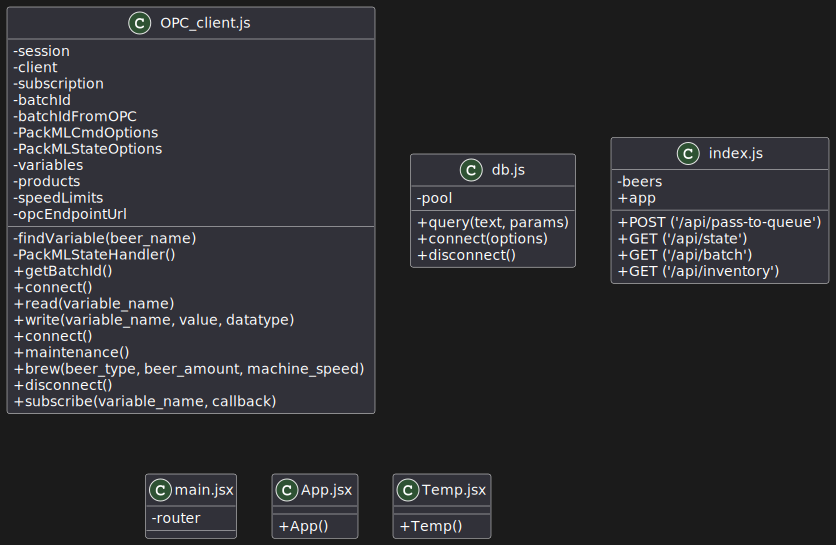
\includegraphics[width=1\textwidth]{img/class_diagram.png}
        \caption{Class diagram of the system}
        \label{fig:class_diagram}
    \end{figure}
\end{center}
Figure \ref{fig:class_diagram} shows the class diagram of the system. The diagram shows the different classes and how they are connected. The system is divided into three components, a dockerfile that boots up the backend, frontend and OPCUA-Client, we have the beer machine itself, and lastly the database which enables us to save data that is generated during the brewing process. This data collected can be accesed and help us understand and give improvements to the system.

\subsubsubsection{index.js}

The index.js file is responsible for our backend, which handles routing and requests. Currently we have the following endpoints;
\begin{enumerate}
    \item {POST ('/api/pass-to-queue')}
    \item {GET ('/api/state')}
    \item {GET ('/api/inventory')}
\end{enumerate}

Our only \textit{POST} endpoint, which is the first on the list, is responsible for creating a brewing order. It recevies a body of type JSON with the keys \textit{'speed'},\textit{'amount'} and \textit{'type'}, which is the beer type. However the speed is not required. If there isn't any value entered, it will have a fallback of the optimal machine speed.
While running the brewing method, it will continously update the state, as we have subscribed to the Node, that holds the stateCurrent value. If it isn't in \textit{execute}, which is the state that it is in, when it is brewing, it will brew. Otherwise if it is brewing (in execute state or 6 of value), then it will send an error to the user and not run that brewing order.
This way it can never brew if it is already brewing. \newline

Our 3 \textit{GET} endpoints is just for the client to receive data. Which is the state and inventory, respectively.
All of these \textit{GET} endpoints are server-sent events (SSE). This means that the user will get the information streamed down continously. \newline

Our most essential API endpoint is our POST request, as it is the one to make a brewing order. Here is some of our code to show what is happening, when a user makes an order;

\begin{center}
    \centering
    \begin{figure}[H]
        \begin{minted}[tabsize=2,breaklines]{javascript}
            app.post('/api/pass-to-queue', async (req, res) => {
                try {
                    // input validation code...
                    await opcuaClient.connect()
        
                    const state = opcuaClient.getStateCurrent()
                    if (state == opcuaClient.PackMLStateOptions.Execute) throw new Error('Brewing is not possible at the moment')
        
                    if (await opcuaClient.brew(beer_type, beer_amount, speed ?? 10)) {
                        // send beer type request to queue
                        res.status(200) // if ok, return status code OK
                        res.send({ status: 'ok' })
                    } else {
                        res.status(418) // refuse to brew
                        res.send({ status: 'error', error: 'Brewing failed' })
                    }
                } catch (error) {
                    console.error(error)
                    res.status(500).send({ error: error.message, status: 'error' })
                }
            })
        \end{minted}
        \caption{Code for our \textit{POST} endpoint}
        \label{fig:pass_to_queue_api}
    \end{figure}
\end{center}
Figure \ref{fig:pass_to_queue_api} shows the code for our \textit{POST} endpoint. It is responsible for making a brewing order. It first checks if the state is in \textit{execute}, which is the state it is in, when it is brewing. If it is, then it will throw an error, as it is not possible to brew, when it is already brewing. Otherwise, it will brew the beer, and if it is successful, it will send a status code of 200, which means OK. Otherwise, it will send a status code of 418, which means I'm a teapot. This is just a joke. But it is a valid status code, so we decided to use it.

\subsubsubsection{OPC\_client.js}


\begin{center}
    \centering
    \begin{figure}[H]
        \begin{minted}[tabsize=2,breaklines,breakanywhere,samepage]{javascript}
            brew: async (beer_type, beer_amount, machine_speed) => {
                try {
                    if (beer_type === undefined || !beer_amount || !machine_speed) return false                    

                    if (Object.values(products).indexOf(beer_type) === -1) return false

                    const maxMachineSpeedForBeerType = speedLimits[beer_type]

                    if (machine_speed < 0 || machine_speed > maxMachineSpeedForBeerType) return false

                    ... 

                    let state = await module.exports.read('StateCurrent')
                    if (state !== PackMLStateOptions.Execute) await PackMLStateHandler()

                    const currentStopReason = await module.exports.read('StopReason')
                    const needsMaintenance = currentStopReason === 10 || currentStopReason === 11

                    if (needsMaintenance) await module.exports.maintenence()

                    for (let node of nodesToWrite) {
                        const StopReason = await module.exports.read('StopReason')
                        if (StopReason === 10 || StopReason === 11) await module.exports.maintenence()
                        await module.exports.write(node.variable, node.value, node.dataType)
                    }

                    batchId++
                    await module.exports.write('SetBatchId', batchId, DataType.Float)

                    state = await module.exports.read('StateCurrent')
                    if (state !== PackMLStateOptions.Execute) await PackMLStateHandler()
                    return true
                } catch (err) {
                    console.error('An error occurred while brewing:', err)
                    return false
                }
            },
        \end{minted}
        \caption{Code for our brew method}
        \label{fig:opc_client_brew}
    \end{figure}
\end{center}
Figure \ref{fig:opc_client_brew} shows the code for our beer brewing method. Initially, it validates essential parameters—beer type, amount, and machine speed—returning false if any are undefined or set to zero. Furthermore, it confirms the beer type's existence in the products object and checks if the machine speed falls within the acceptable range for that type. \newline

After these checks, it ensures the system is in the 'execute' state for brewing. If not, it triggers the PackMLStateHandler method. It also handles maintenance if the stop reason is 10 or 11, iterating through nodesToWrite to update data.\newline

Upon successful execution, it returns true. Any encountered errors prompt a false return.\newline